\documentclass[11pt,a4paper]{article}

% =========================================================
% NetFix Unified Platform -- User Guide
% Standalone document; not part of the thesis template
% =========================================================

% ---------------------------------------------------------
% Packages
% ---------------------------------------------------------
\usepackage[utf8]{inputenc}
\usepackage[T1]{fontenc}
\usepackage[a4paper,top=0.72in,bottom=0.72in,left=0.78in,right=0.78in]{geometry}
\usepackage{amsmath,amssymb}
\usepackage{graphicx}
\usepackage{xcolor}
\usepackage{booktabs}
\usepackage{tabularx}
\usepackage{array}
\usepackage{multirow}
\usepackage{enumitem}
\usepackage{microtype}
\usepackage{parskip}
\usepackage{fancyhdr}
\usepackage{titlesec}
\usepackage{caption}
\usepackage{subcaption}
\usepackage{float}
\usepackage{placeins}
\usepackage[most]{tcolorbox}
\usepackage{hyperref}
\usepackage{xurl}

\graphicspath{{Figures/}}

% ---------------------------------------------------------
% Visual identity
% ---------------------------------------------------------
\definecolor{netfixBlue}{RGB}{21,101,192}
\definecolor{netfixNavy}{RGB}{21,37,73}
\definecolor{netfixCyan}{RGB}{0,172,193}
\definecolor{netfixMagenta}{RGB}{198,24,93}
\definecolor{netfixGreen}{RGB}{32,130,82}
\definecolor{netfixOrange}{RGB}{230,126,34}
\definecolor{netfixRed}{RGB}{198,40,40}
\definecolor{softBlue}{RGB}{241,247,253}
\definecolor{softGray}{RGB}{247,249,252}
\definecolor{midGray}{RGB}{92,108,126}
\definecolor{ruleGray}{RGB}{218,226,235}

\hypersetup{
  colorlinks=true,
  linkcolor=netfixBlue,
  urlcolor=netfixBlue,
  citecolor=netfixBlue,
  pdftitle={NetFix Unified Platform User Guide},
  pdfauthor={NetFix Core Engineering Team}
}

% ---------------------------------------------------------
% Typography and layout
% ---------------------------------------------------------
\setlength{\parindent}{0pt}
\setlength{\parskip}{4.5pt}
\renewcommand{\arraystretch}{1.18}
\setlength{\tabcolsep}{5pt}
\emergencystretch=2em

\setlist[itemize]{leftmargin=1.0cm,itemsep=2pt,topsep=3pt,parsep=0pt}
\setlist[enumerate]{leftmargin=1.05cm,itemsep=3pt,topsep=3pt,parsep=0pt}

\titleformat{\section}
  {\normalfont\Large\bfseries\color{netfixNavy}}
  {\thesection}{0.65em}{}
\titlespacing*{\section}{0pt}{16pt}{7pt}

\titleformat{\subsection}
  {\normalfont\large\bfseries\color{netfixBlue}}
  {\thesubsection}{0.6em}{}
\titlespacing*{\subsection}{0pt}{13pt}{5pt}

\titleformat{\subsubsection}
  {\normalfont\normalsize\bfseries\color{netfixNavy}}
  {\thesubsubsection}{0.55em}{}
\titlespacing*{\subsubsection}{0pt}{9pt}{3pt}

\captionsetup{
  font=small,
  labelfont={bf,color=netfixNavy},
  textfont={color=netfixNavy},
  justification=centering,
  singlelinecheck=false,
  skip=5pt
}

\newcolumntype{Y}{>{\raggedright\arraybackslash}X}
\newcolumntype{L}[1]{>{\raggedright\arraybackslash}p{#1}}

% ---------------------------------------------------------
% Header / footer
% ---------------------------------------------------------
\pagestyle{fancy}
\fancyhf{}
\lhead{\small\bfseries\color{netfixBlue}NetFix Unified Platform}
\rhead{\small\color{midGray}User Guide}
\cfoot{\color{midGray}\thepage}
\renewcommand{\headrulewidth}{0.35pt}
\renewcommand{\footrulewidth}{0pt}
\setlength{\headheight}{15pt}

% ---------------------------------------------------------
% Reusable guide boxes
% ---------------------------------------------------------
\tcbset{
  enhanced,
  breakable,
  boxrule=0.6pt,
  arc=2mm,
  left=7pt,right=7pt,top=6pt,bottom=6pt
}

\newtcolorbox{guidebox}[1]{
  title=#1,
  colback=softBlue,
  colframe=netfixBlue,
  coltitle=white,
  fonttitle=\bfseries,
  attach boxed title to top left={xshift=3mm,yshift=-2mm},
  boxed title style={colback=netfixBlue,colframe=netfixBlue,arc=1.5mm},
  top=9pt
}

\newtcolorbox{workflowbox}[1]{
  title=#1,
  colback=softGray,
  colframe=ruleGray,
  coltitle=netfixNavy,
  fonttitle=\bfseries,
  boxed title style={colback=white,colframe=ruleGray},
  attach boxed title to top left={xshift=3mm,yshift=-2mm},
  top=9pt
}

\newtcolorbox{warningbox}[1]{
  title=#1,
  colback=white,
  colframe=netfixOrange,
  coltitle=white,
  fonttitle=\bfseries,
  boxed title style={colback=netfixOrange,colframe=netfixOrange},
  attach boxed title to top left={xshift=3mm,yshift=-2mm},
  top=9pt
}

% ---------------------------------------------------------
% Document
% ---------------------------------------------------------
\begin{document}

% =========================================================
% Cover
% =========================================================
\begin{titlepage}
\thispagestyle{empty}
\centering
\vspace*{1.5cm}

{\color{netfixBlue}\rule{0.22\textwidth}{1.2pt}}\hspace{0.4cm}
{\color{netfixMagenta}\rule{0.08\textwidth}{1.2pt}}\hspace{0.4cm}
{\color{netfixBlue}\rule{0.22\textwidth}{1.2pt}}

\vspace{1.1cm}
{\fontsize{30}{34}\selectfont\bfseries\color{netfixNavy}NetFix Unified Platform}\par
\vspace{0.3cm}
{\fontsize{19}{23}\selectfont\bfseries\color{netfixBlue}Technical User Guide}\par
\vspace{0.4cm}
{\large\color{midGray}Drive Test Intelligence \textbullet\ Root Cause Analysis \textbullet\ 5G Planning Intelligence}\par

\vspace{1.35cm}
\begin{tcolorbox}[
  width=0.86\textwidth,
  colback=softBlue,
  colframe=netfixBlue,
  boxrule=0.8pt,
  arc=3mm,
  left=12pt,right=12pt,top=12pt,bottom=12pt]
\centering
\textbf{Purpose}\par
\vspace{2pt}
This guide explains how optimization and planning engineers use the NetFix web platform: sign in, load data, run analysis, inspect evidence, use AI-assisted workflows, review geospatial results, and export engineering outputs.
\end{tcolorbox}

\vfill
{\large\bfseries NetFix Core Engineering Team}\par
\vspace{0.2cm}
{\color{midGray}\today}\par
\vspace{0.8cm}
{\color{ruleGray}\rule{0.88\textwidth}{0.6pt}}
\end{titlepage}

\tableofcontents
\newpage

% =========================================================
\section{Platform Overview and Role-Based Routing}
% =========================================================
The \textbf{NetFix Unified Telecommunication Platform} brings two independent engineering workspaces into one web application:

\begin{guidebox}{Two engineering workspaces}
\textbf{Drive Test Intelligence / Anomaly Portal} combines statistical anomaly detection, Histogram Gradient Boosting ML, PyTorch LSTM temporal validation, a 34-reason deterministic Root Cause Analysis (RCA) engine, interactive Leaflet GIS mapping, and the local \textbf{Penguin AI} assistant.

\medskip
\textbf{5G Planning Intelligence / NetPulse} performs spatial geometry analysis, neighbor-graph validation, and constraint-based planning of 5G NR PCI, RSI, and PRACH parameters while enforcing Mod3, Mod4, and Mod30 conflict rules.
\end{guidebox}

The datasets used by these workspaces are handled independently. The common platform layer provides authentication, role routing, user experience, persistence, reporting, and AI-assisted interaction.

\subsection{Role-based routing}
\begin{itemize}
  \item \textbf{Optimization Engineer} $\rightarrow$ Drive Test Intelligence dashboard at \texttt{/dashboard}.
  \item \textbf{Planning Engineer} $\rightarrow$ NetPulse Upload \& Plan workspace at \texttt{/np-upload}.
\end{itemize}

\begin{workflowbox}{Quick start}
\textbf{Optimization workflow:} Sign in $\rightarrow$ Upload dataset $\rightarrow$ Wait for the four pipeline stages $\rightarrow$ Review dashboard $\rightarrow$ Open an incident $\rightarrow$ Run RCA $\rightarrow$ Inspect map / Penguin AI / report.

\medskip
\textbf{Planning workflow:} Sign in $\rightarrow$ Upload workbook $\rightarrow$ Inspect clashes $\rightarrow$ Bulk replan or add a site $\rightarrow$ Validate assignments $\rightarrow$ Export the final workbook.
\end{workflowbox}

\newpage

% =========================================================
\section{Drive Test Intelligence and Troubleshooting Portal}
% =========================================================
\begin{guidebox}{Target user: Optimization Engineer / RF Performance Specialist}
This section documents the operational workflow of the NetFix anomaly-detection and RCA portal, including navigation, telemetry monitoring, dataset ingestion, deterministic RCA, GIS inspection, AI-assisted analysis, reporting, and session history.
\end{guidebox}

\subsection{Navigation and workspace layout}
The portal uses a persistent dark navigation sidebar and a light analysis workspace. The main entries are:

\begin{itemize}
  \item \textbf{Dashboard} --- telemetry overview, KPI cards, severity distribution, and backend validation figures.
  \item \textbf{Upload Dataset} --- raw \texttt{.pkl} ingestion, four-stage progress tracking, and recent-session audit.
  \item \textbf{Results} --- deterministic RCA, telemetry evidence, standards references, and recommended actions.
  \item \textbf{Interactive Map} --- Leaflet GIS trajectory, cell/tower context, and anomaly markers.
  \item \textbf{Reports} --- diagnostic summaries and exported analysis outputs.
  \item \textbf{Penguin AI} --- local LLM engineering copilot for grounded analysis and report generation.
  \item \textbf{History} --- historical sessions, completion states, anomaly counts, and cause-matching status.
  \item \textbf{Settings} --- threshold defaults, model preferences, and API configuration.
\end{itemize}

The bottom-left user badge shows the authenticated engineer, current role, and logout controls.

% ---------------------------------------------------------
\subsection{Module 1: Telemetry Overview and ML Pipeline Dashboard}
% ---------------------------------------------------------
The Dashboard is the primary landing page after authentication. It gives an immediate view of the active dataset and provides direct access to generated backend figures (Figure~\ref{fig:ug-dashboard}).

\begin{figure}[H]
\centering
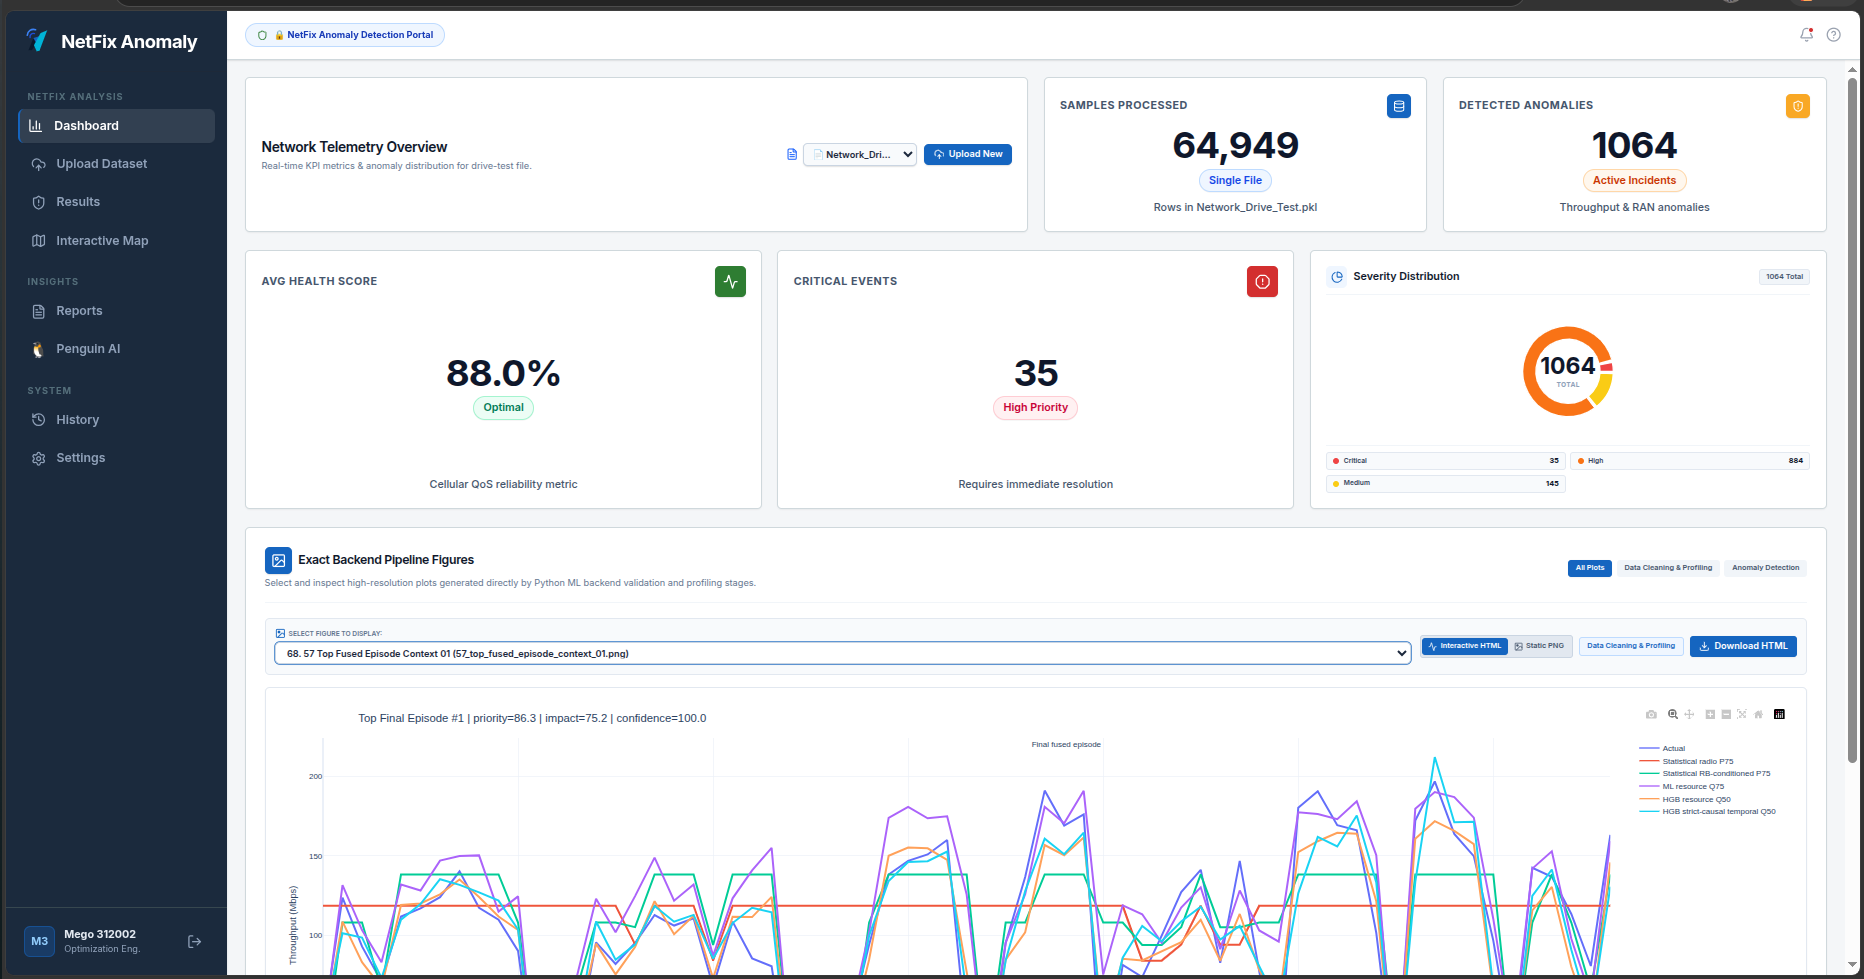
\includegraphics[width=0.96\textwidth]{Screenshot from 2026-08-12 14-38-38.png}
\caption{Telemetry dashboard with dataset metrics, incident severity distribution, and backend analysis figures.}
\label{fig:ug-dashboard}
\end{figure}
\FloatBarrier

\subsubsection{Top telemetry metrics}
\begin{table}[H]
\centering
\small
\begin{tabularx}{0.97\textwidth}{L{3.3cm} L{2.2cm} Y}
\toprule
\textbf{Metric} & \textbf{Displayed value} & \textbf{Meaning} \\
\midrule
Samples Processed & \textbf{64,949} & Total telemetry rows loaded from \texttt{Network\_Drive\_Test.pkl}. \\
Detected Anomalies & \textbf{1,064} & Active incident episodes retained for RCA analysis and platform review. \\
Average Health Score & \textbf{88.0\%} & Cellular QoS reliability indicator shown with an \texttt{Optimal} status. \\
Critical Events & \textbf{35} & Highest-priority operational cases requiring immediate engineering attention. \\
\bottomrule
\end{tabularx}
\caption{Dashboard telemetry summary.}
\label{tab:dash-metrics-ug}
\end{table}

\subsubsection{Severity distribution}
The incident donut chart separates the 1,064 displayed incidents into:
\begin{itemize}
  \item \textbf{Critical: 35} --- severe throughput degradation or radio-link failure conditions.
  \item \textbf{High: 884} --- significant degradation relative to expected performance.
  \item \textbf{Medium: 145} --- moderate KPI variance or localized degradation.
\end{itemize}

\subsubsection{Backend figure viewer}
The figure panel exposes the exact plots produced by the Python analysis pipeline. Engineers can select an artifact, switch between interactive HTML and static PNG when available, and download the corresponding HTML output. Typical throughput-context figures compare:
\begin{itemize}
  \item actual throughput;
  \item radio-conditioned statistical P75;
  \item RB-conditioned statistical P75;
  \item ML resource Q75;
  \item HGB resource-conditioned central prediction; and
  \item HGB strict-causal temporal central prediction.
\end{itemize}

% ---------------------------------------------------------
\subsection{Module 2: Dataset Ingestion and Four-Stage Execution}
% ---------------------------------------------------------
The Upload Dataset page controls ingestion and exposes pipeline status in real time (Figure~\ref{fig:ug-upload}).

\begin{figure}[H]
\centering
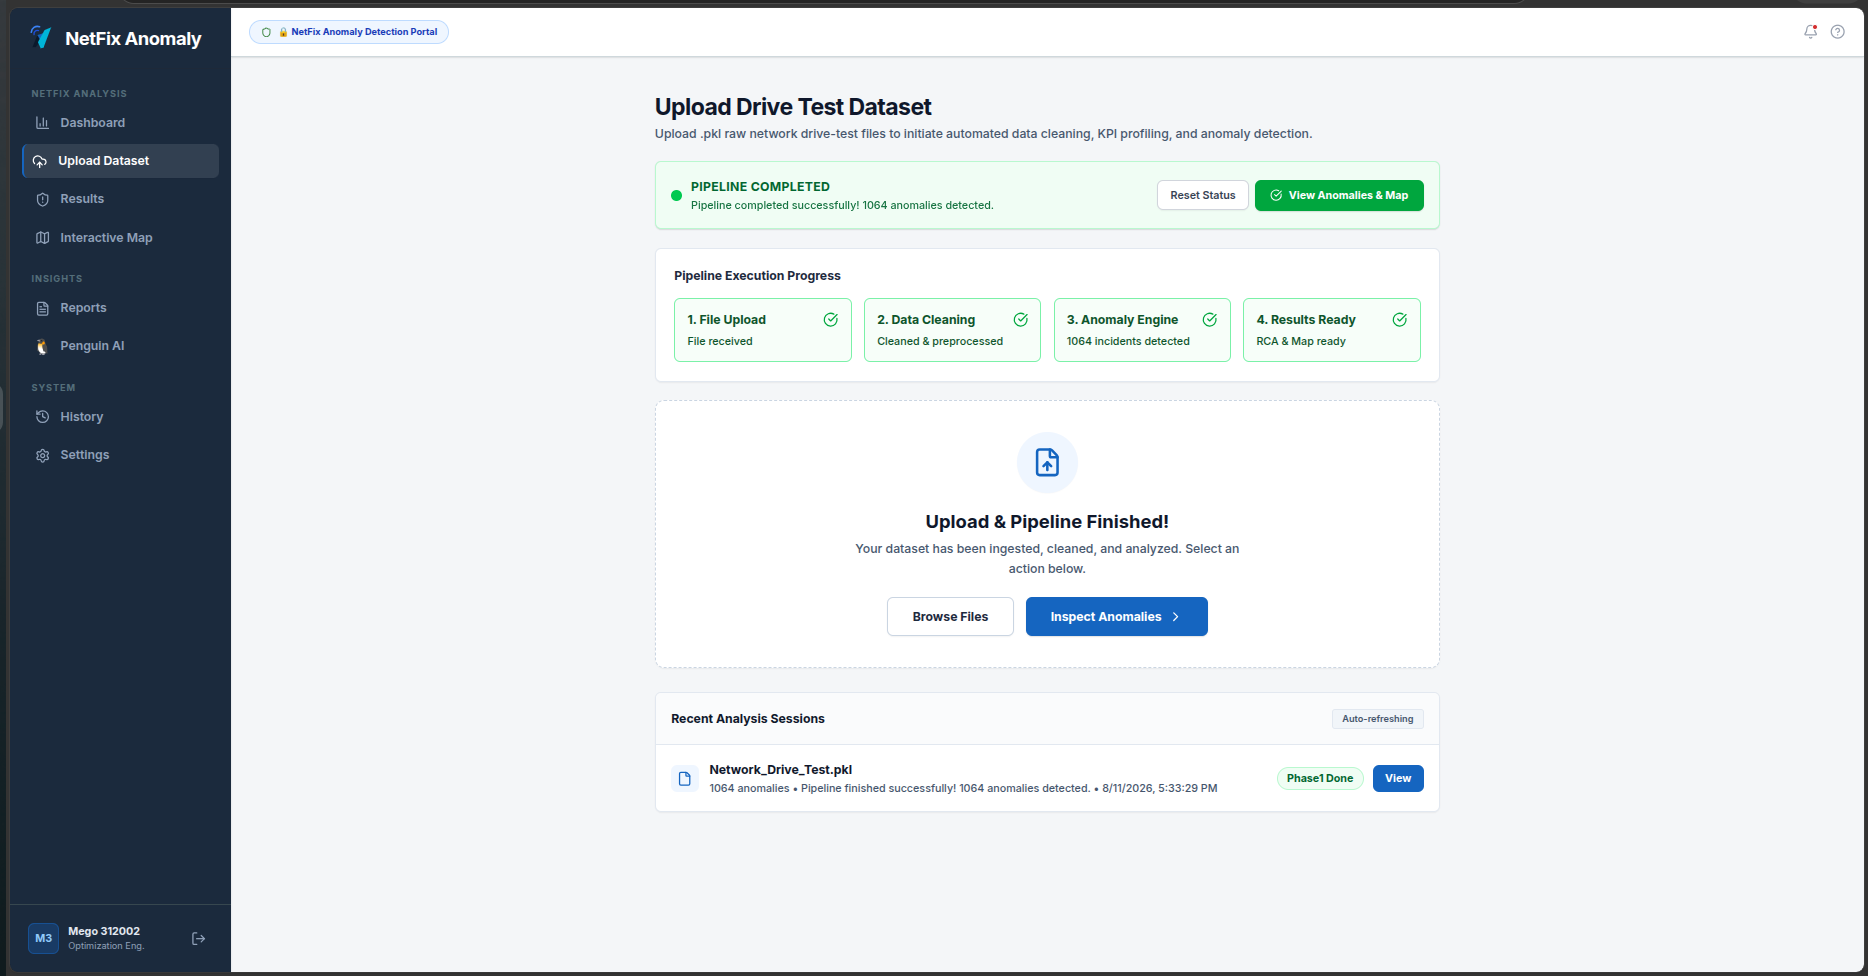
\includegraphics[width=0.96\textwidth]{Screenshot from 2026-08-12 14-38-48.png}
\caption{Dataset upload workflow with four-stage execution status and recent analysis sessions.}
\label{fig:ug-upload}
\end{figure}
\FloatBarrier

\subsubsection{Execution stages}
\begin{enumerate}
  \item \textbf{File Upload} --- validates the payload and receives the raw \texttt{.pkl} drive-test file.
  \item \textbf{Data Cleaning} --- executes the 11-stage non-leaking preprocessing pipeline (\texttt{ran-cleaning-}\allowbreak\texttt{service}).
  \item \textbf{Anomaly Engine} --- runs the 19-stage statistical, HGB ML, and PyTorch LSTM anomaly-fusion workflow.
  \item \textbf{Results Ready} --- builds MongoDB session indexes and prepares RCA cause matching and GIS artifacts.
\end{enumerate}

On success, the page confirms pipeline completion and the incident count. \textbf{View Anomalies \& Map} opens the investigation workspace; \textbf{Reset Status} prepares the interface for a new upload.

The Recent Analysis Sessions table records dataset name, anomaly count, timestamp, pipeline state, and a direct session-view action.

% ---------------------------------------------------------
\subsection{Module 3: Deterministic RCA Engine and Telemetry Evidence}
% ---------------------------------------------------------
The Results workspace is used to select an incident, run deterministic RCA, inspect telemetry evidence, review AI-supported engineering interpretation, and follow recommended actions. Figures~\ref{fig:ug-rca-grid} and~\ref{fig:ug-rca-recs} show the two main views.

\begin{figure}[H]
\centering
\begin{subfigure}[t]{0.49\textwidth}
  \centering
  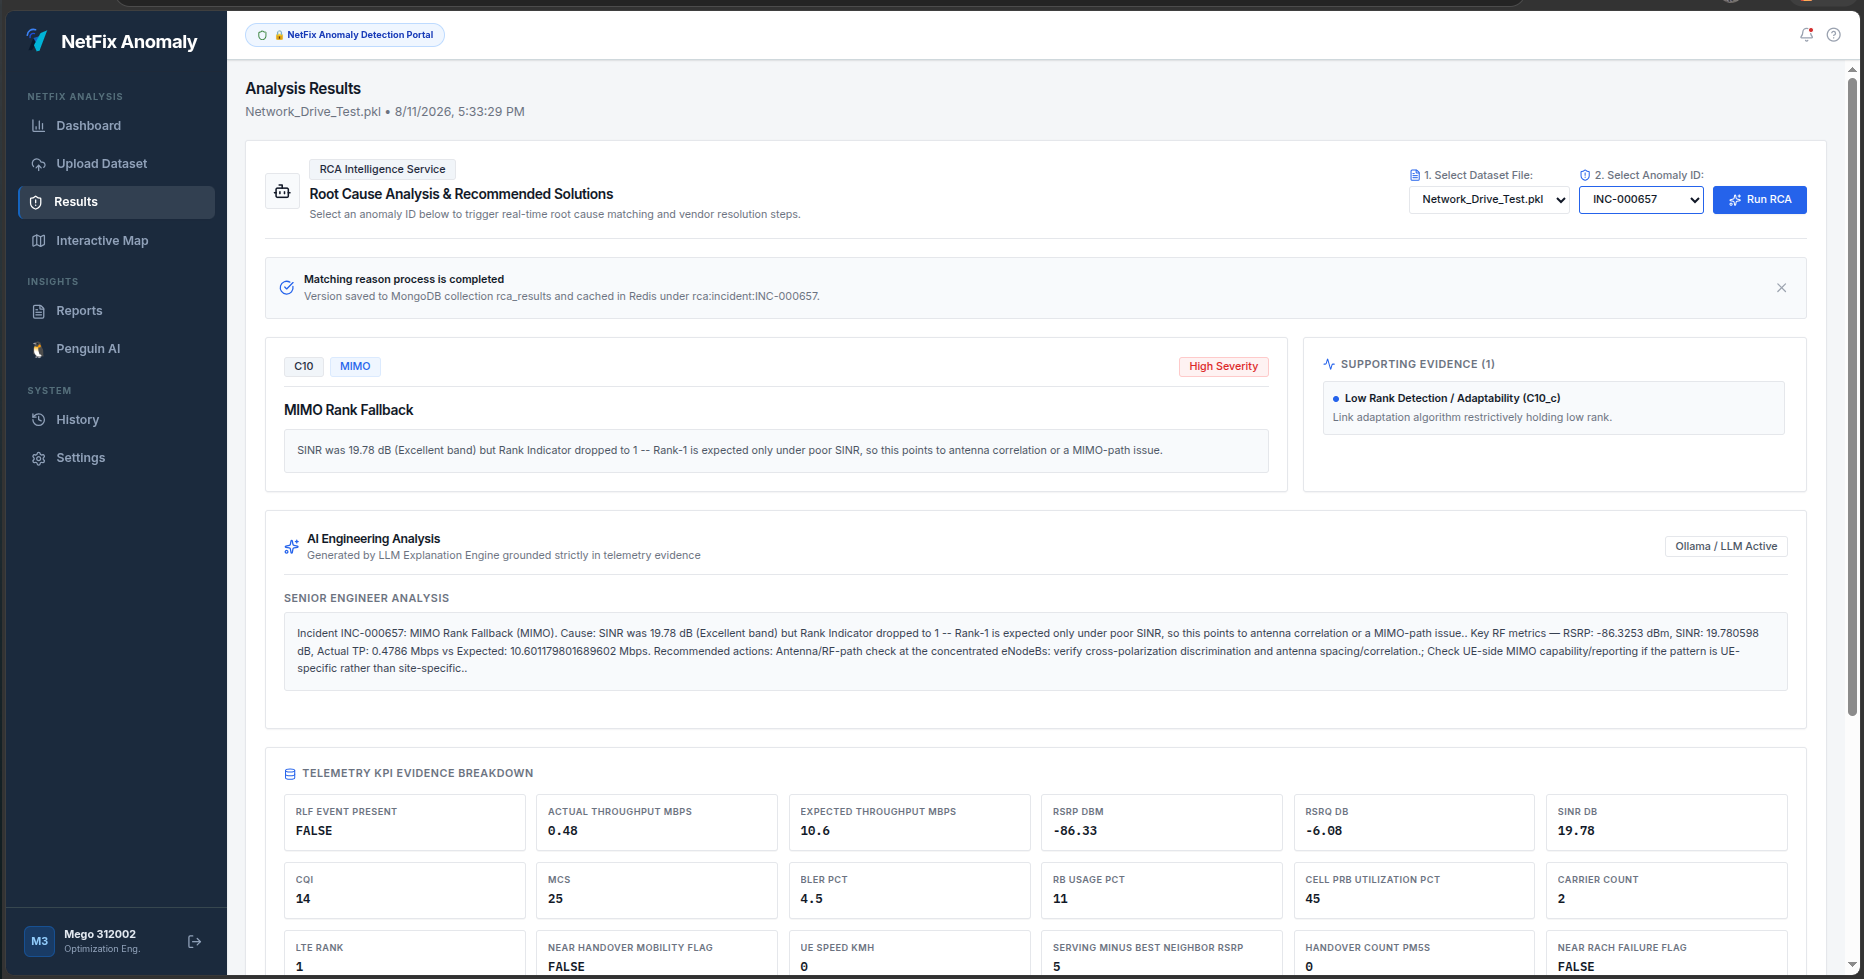
\includegraphics[width=\linewidth]{Screenshot from 2026-08-12 14-39-04.png}
  \caption{Matched RCA rule, AI engineering analysis, and telemetry evidence grid.}
  \label{fig:ug-rca-grid}
\end{subfigure}\hfill
\begin{subfigure}[t]{0.49\textwidth}
  \centering
  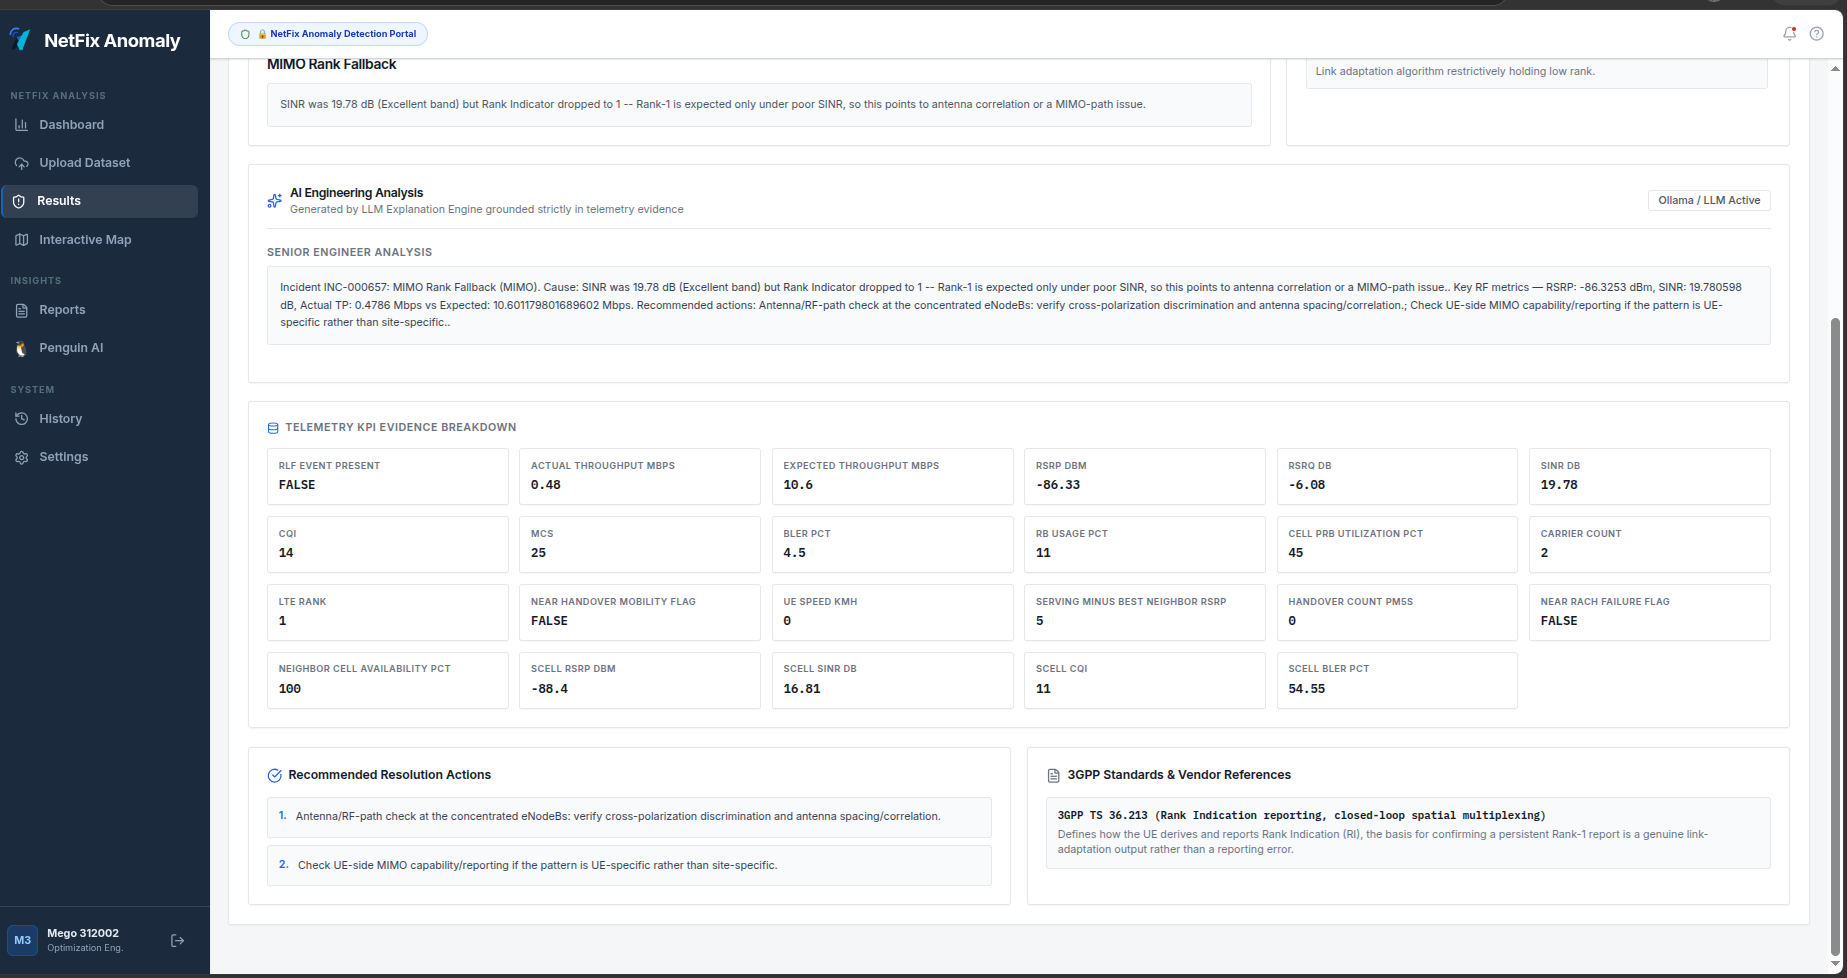
\includegraphics[width=\linewidth]{Screenshot from 2026-08-12 14-39-08.png}
  \caption{Recommended actions and 3GPP standards reference.}
  \label{fig:ug-rca-recs}
\end{subfigure}
\caption{Deterministic RCA workflow for an individual incident.}
\label{fig:ug-rca-workflow}
\end{figure}
\FloatBarrier

\subsubsection{Incident selection and execution}
Select the dataset and Incident ID (for example, \texttt{INC-000657}), then click \textbf{Run RCA}. The completion banner confirms that the matched-reason process has finished, saves the result to MongoDB collection \texttt{rca\_results}, and caches the incident in Redis under the corresponding incident key.

\subsubsection{Example rule match: MIMO Rank Fallback}
For \texttt{INC-000657}, the portal shows:
\begin{itemize}
  \item \textbf{Category / severity:} \texttt{C10}, \texttt{MIMO}, High Severity.
  \item \textbf{Matched reason:} \textbf{MIMO Rank Fallback}.
  \item \textbf{Reasoning:} SINR is 19.78 dB while Rank Indicator falls to 1; Rank-1 under strong SINR suggests antenna correlation or a MIMO-path problem rather than weak RF conditions.
  \item \textbf{Supporting evidence:} low-rank adaptation remains active despite clean RF conditions.
\end{itemize}

\subsubsection{AI engineering interpretation}
The local Ollama analysis card combines the deterministic rule with the actual telemetry. In the illustrated incident it reports RSRP $=-86.3253$ dBm, SINR $=19.780598$ dB, actual throughput $=0.4786$ Mbps, and expected throughput $=10.601179$ Mbps. The recommended engineering checks focus on antenna / RF-path behavior, cross-polarization discrimination, spacing / correlation, and UE-side MIMO capability when the pattern appears UE-specific.

\subsubsection{23-metric telemetry evidence}
\begin{table}[H]
\centering
\scriptsize
\begin{tabularx}{0.98\textwidth}{L{4.5cm} L{3.0cm} Y}
\toprule
\textbf{Telemetry field} & \textbf{Recorded value} & \textbf{Evaluation} \\
\midrule
RLF EVENT PRESENT & FALSE & No Radio Link Failure event. \\
ACTUAL THROUGHPUT MBPS & 0.48 Mbps & Severe degradation; expected throughput is 10.6 Mbps. \\
EXPECTED THROUGHPUT MBPS & 10.6 Mbps & Calculated P75 baseline for the cell/context. \\
RSRP DBM & -86.33 dBm & Good serving-cell signal strength. \\
RSRQ DB & -6.08 dB & Good serving-cell signal quality. \\
SINR DB & 19.78 dB & Excellent signal-to-interference ratio. \\
CQI & 14 & High Channel Quality Indicator. \\
MCS & 25 & High Modulation and Coding Scheme index. \\
BLER PCT & 4.5\% & Low Block Error Rate. \\
RB USAGE PCT & 11\% & Low Resource Block usage. \\
CELL PRB UTILIZATION PCT & 45\% & Moderate cell load. \\
CARRIER COUNT & 2 & Dual component carrier; CA active. \\
LTE RANK & 1 & Anomalous under 19.78 dB SINR. \\
NEAR HANDOVER MOBILITY FLAG & FALSE & Stationary / low-mobility state. \\
UE SPEED KMH & 0 km/h & Stationary UE. \\
SERVING MINUS BEST NEIGHBOR RSRP & 5 dB & Adequate cell-dominance margin. \\
HANDOVER COUNT PM5S & 0 & No recent handovers. \\
NEAR RACH FAILURE FLAG & FALSE & Random-access behavior normal. \\
NEIGHBOR CELL AVAILABILITY PCT & 100\% & All neighbor cells available. \\
SCELL RSRP DBM & -88.4 dBm & Secondary-cell RSRP clean. \\
SCELL SINR DB & 16.81 dB & Secondary-cell SINR clean. \\
SCELL CQI & 11 & Secondary-cell CQI acceptable. \\
SCELL BLER PCT & 54.55\% & Secondary-cell BLER elevated. \\
\bottomrule
\end{tabularx}
\caption{Telemetry evidence shown for the example MIMO Rank Fallback incident.}
\label{tab:inc-657-grid-ug}
\end{table}

\subsubsection{Recommended actions and standards grounding}
\begin{enumerate}
  \item Check the antenna / RF path at concentrated eNodeBs, including cross-polarization discrimination and antenna spacing / correlation.
  \item Check UE-side MIMO capability and reporting if the behavior is UE-specific rather than site-specific.
  \item Review \textbf{3GPP TS 36.213} for Rank Indication reporting and closed-loop spatial multiplexing; this standard defines how the UE derives and reports RI.
\end{enumerate}

% ---------------------------------------------------------
\subsection{Module 4: Interactive GIS Trajectory Map}
% ---------------------------------------------------------
The Interactive Map renders the drive-test route and incident locations on a Leaflet canvas (Figure~\ref{fig:ug-map}).

\begin{figure}[H]
\centering
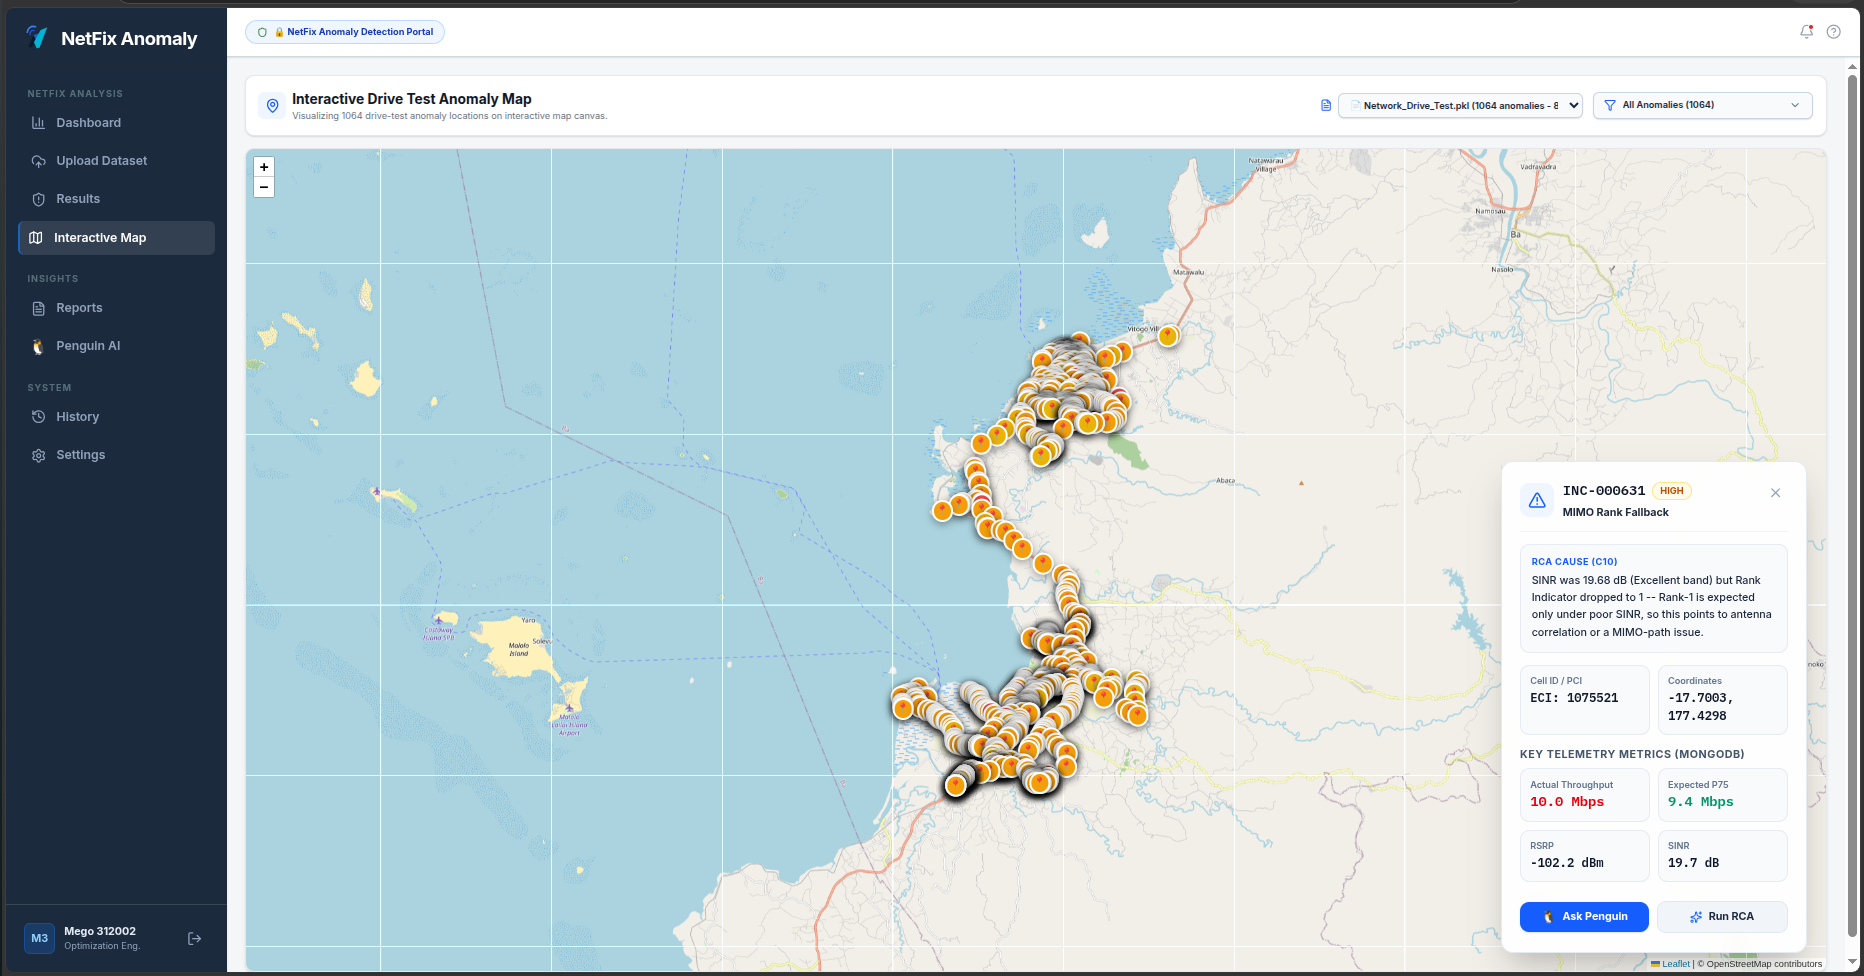
\includegraphics[width=0.96\textwidth]{Screenshot from 2026-08-12 14-39-17.png}
\caption{Drive-test trajectory map with anomaly markers and an incident detail popup.}
\label{fig:ug-map}
\end{figure}
\FloatBarrier

\subsubsection{Controls and inspection workflow}
\begin{itemize}
  \item \textbf{Dataset selector} --- choose the active drive-test dataset.
  \item \textbf{Incident filter} --- display all 1,064 incidents or a selected severity tier.
  \item \textbf{Map navigation} --- pan and zoom over OpenStreetMap tiles.
  \item \textbf{Incident marker} --- open an incident card with severity, reason, serving-cell metadata, coordinates, and selected KPI values.
\end{itemize}

For the illustrated incident \texttt{INC-000631}, the popup identifies a high-severity MIMO Rank Fallback case. The displayed context includes Cell / PCI \texttt{ECI: 1075521}, coordinates \texttt{-17.7003, 177.4298}, actual throughput \textbf{10.0 Mbps}, expected P75 \textbf{9.4 Mbps}, RSRP \textbf{-102.2 dBm}, and SINR \textbf{19.7 dB}. \textbf{Ask Penguin} opens the assistant with the incident context preloaded; \textbf{Run RCA} opens the detailed RCA workspace.

% ---------------------------------------------------------
\subsection{Module 5: Penguin AI Copilot and Report Generator}
% ---------------------------------------------------------
Penguin AI provides a local conversational interface for grounded telecom analysis, incident explanation, KPI relationship reasoning, and structured report generation. Figures~\ref{fig:ug-penguin-chat}--\ref{fig:ug-penguin-cell-edge} illustrate the main interaction modes.

\begin{figure}[H]
\centering
\begin{subfigure}[t]{0.49\textwidth}
  \centering
  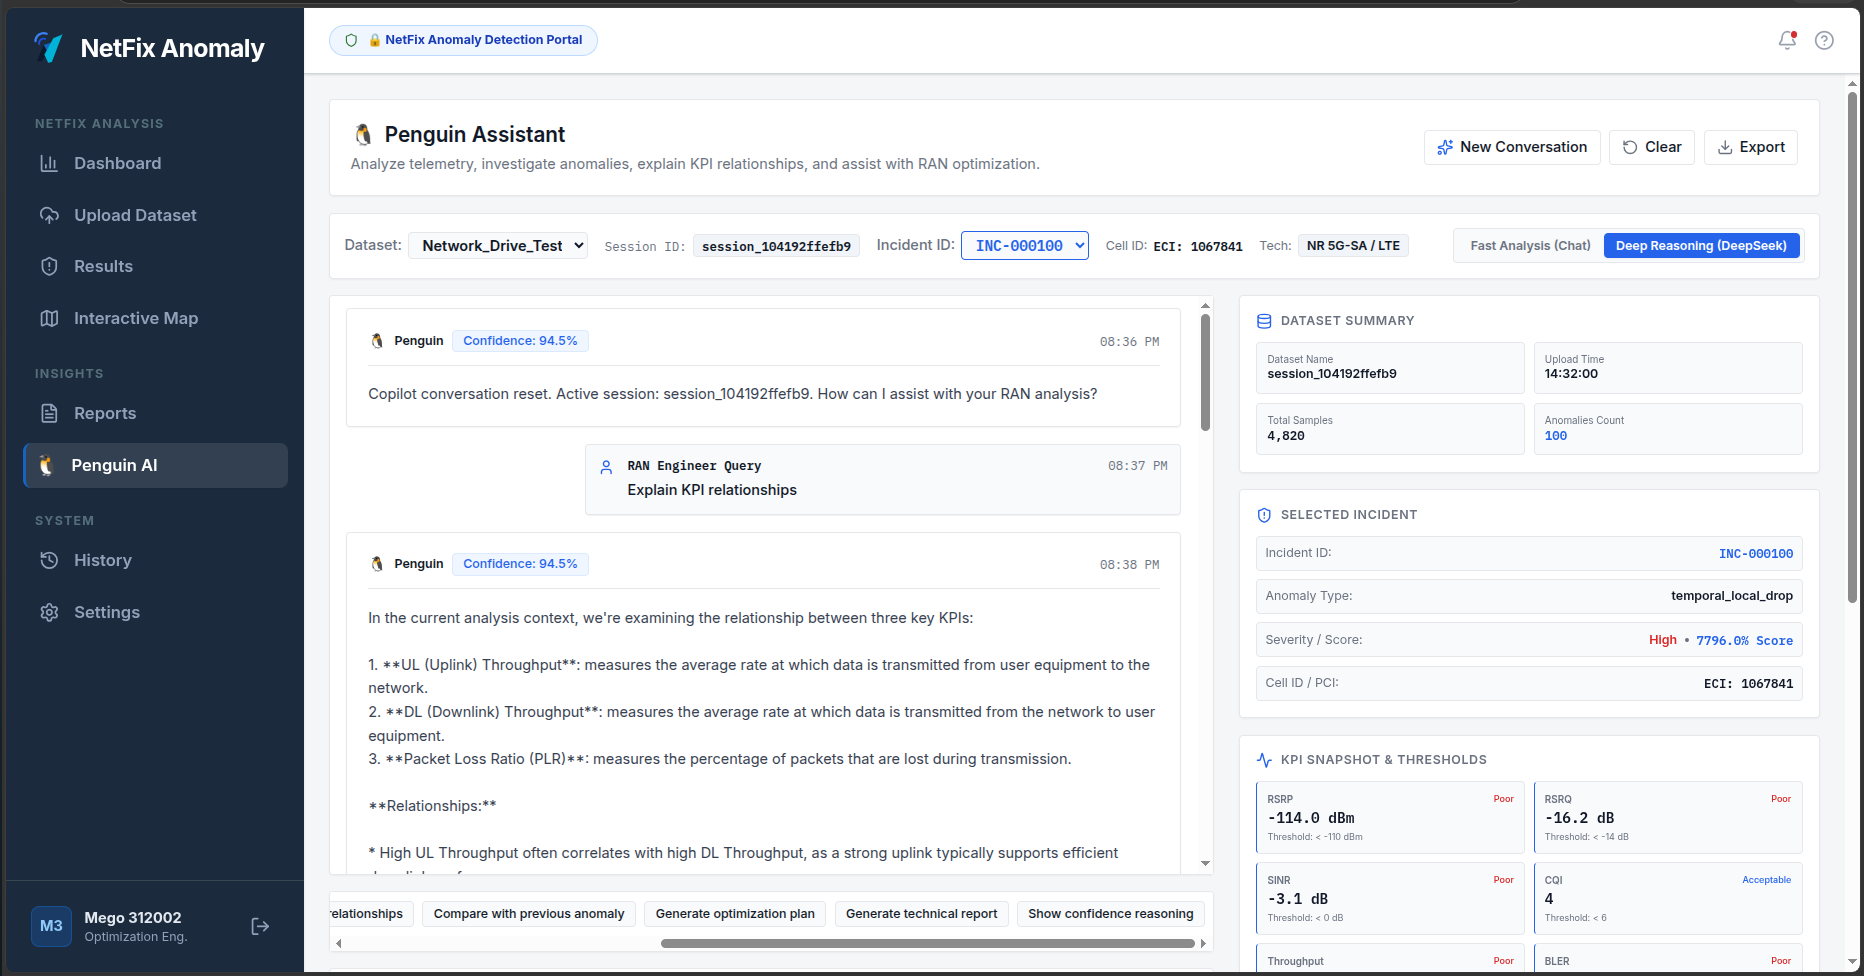
\includegraphics[width=\linewidth]{Screenshot from 2026-08-11 20-52-29.png}
  \caption{KPI relationship explanation with incident context.}
\end{subfigure}\hfill
\begin{subfigure}[t]{0.49\textwidth}
  \centering
  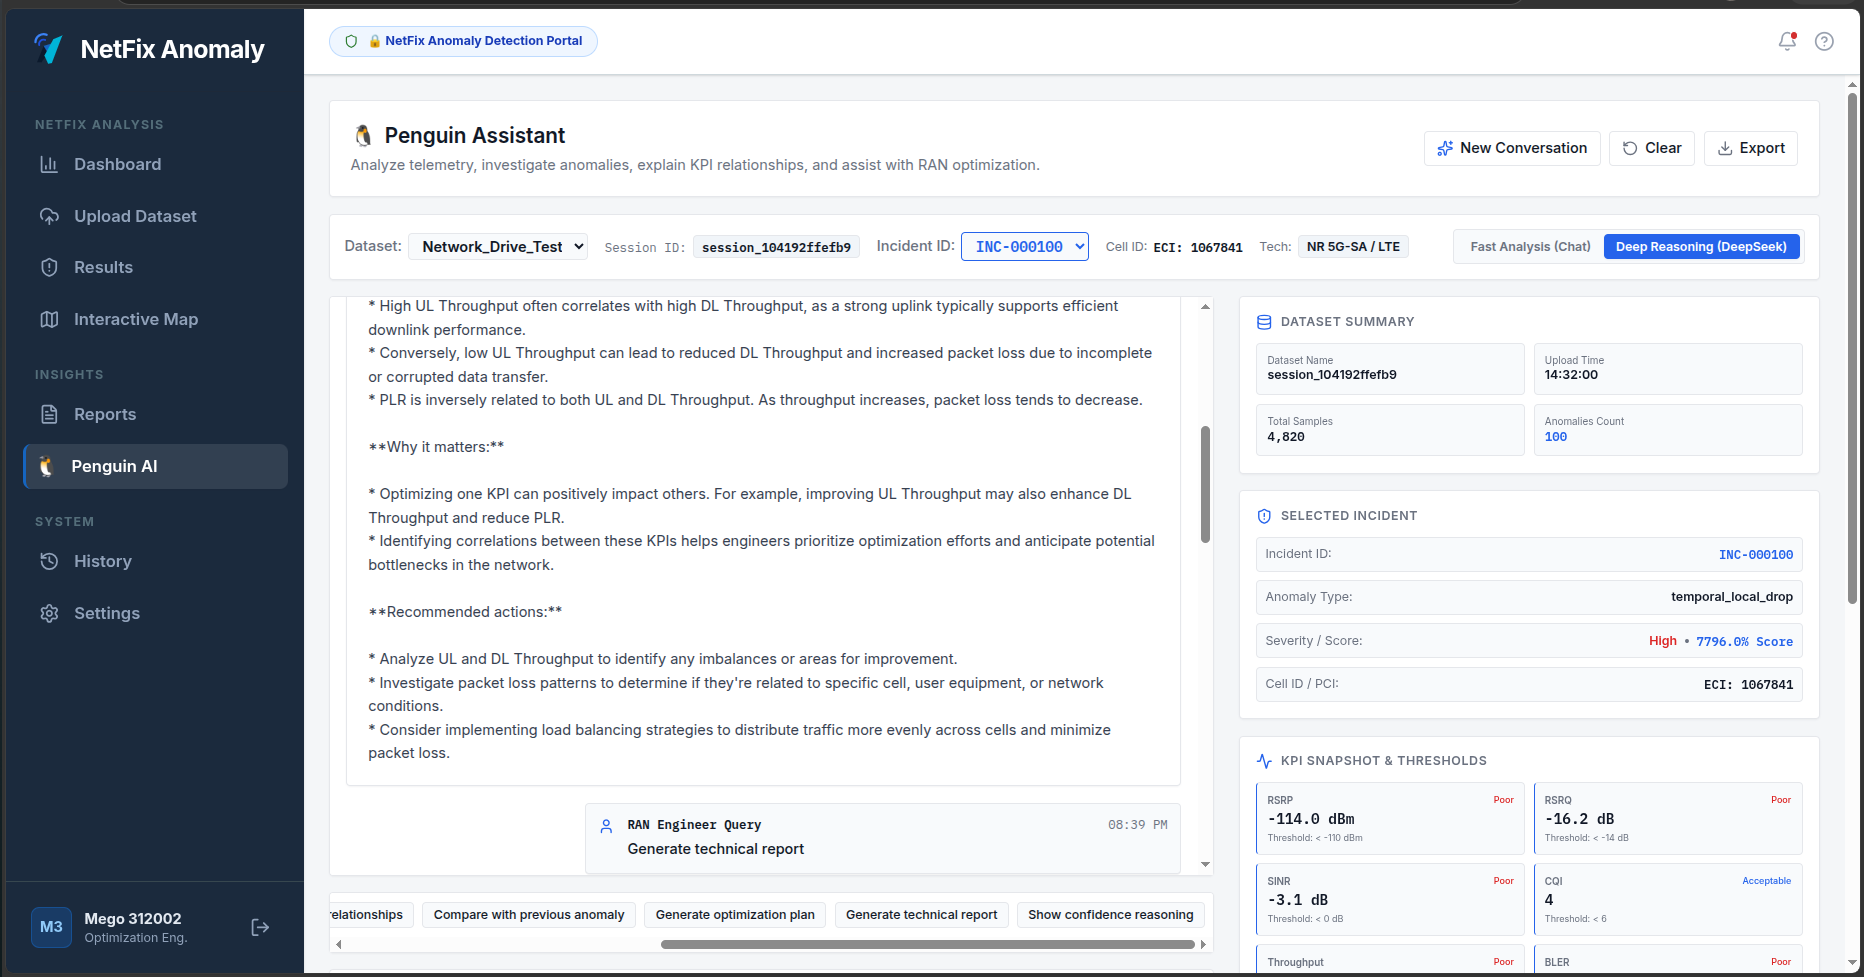
\includegraphics[width=\linewidth]{Screenshot from 2026-08-11 20-52-37.png}
  \caption{Follow-up analysis and quick actions.}
\end{subfigure}
\caption{Penguin AI conversational engineering workflow.}
\label{fig:ug-penguin-chat}
\end{figure}

\begin{figure}[H]
\centering
\begin{subfigure}[t]{0.32\textwidth}
  \centering
  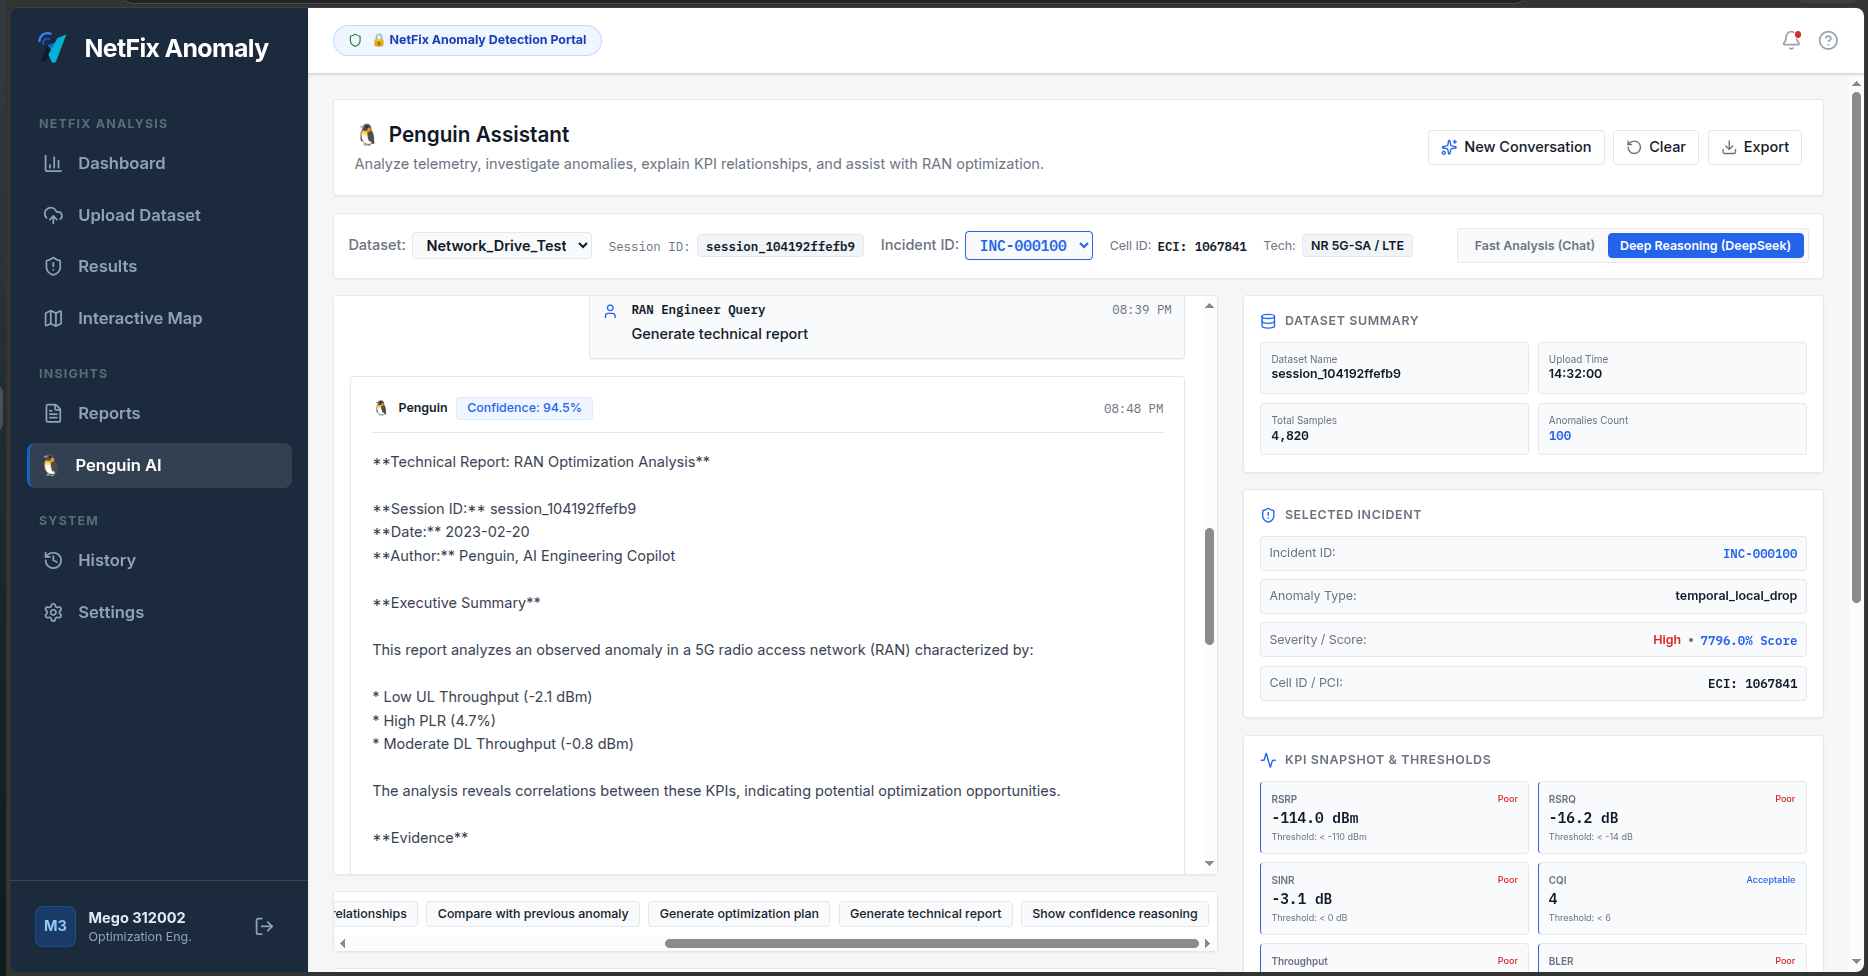
\includegraphics[width=\linewidth]{Screenshot from 2026-08-11 20-52-42.png}
  \caption{Executive summary.}
\end{subfigure}\hfill
\begin{subfigure}[t]{0.32\textwidth}
  \centering
  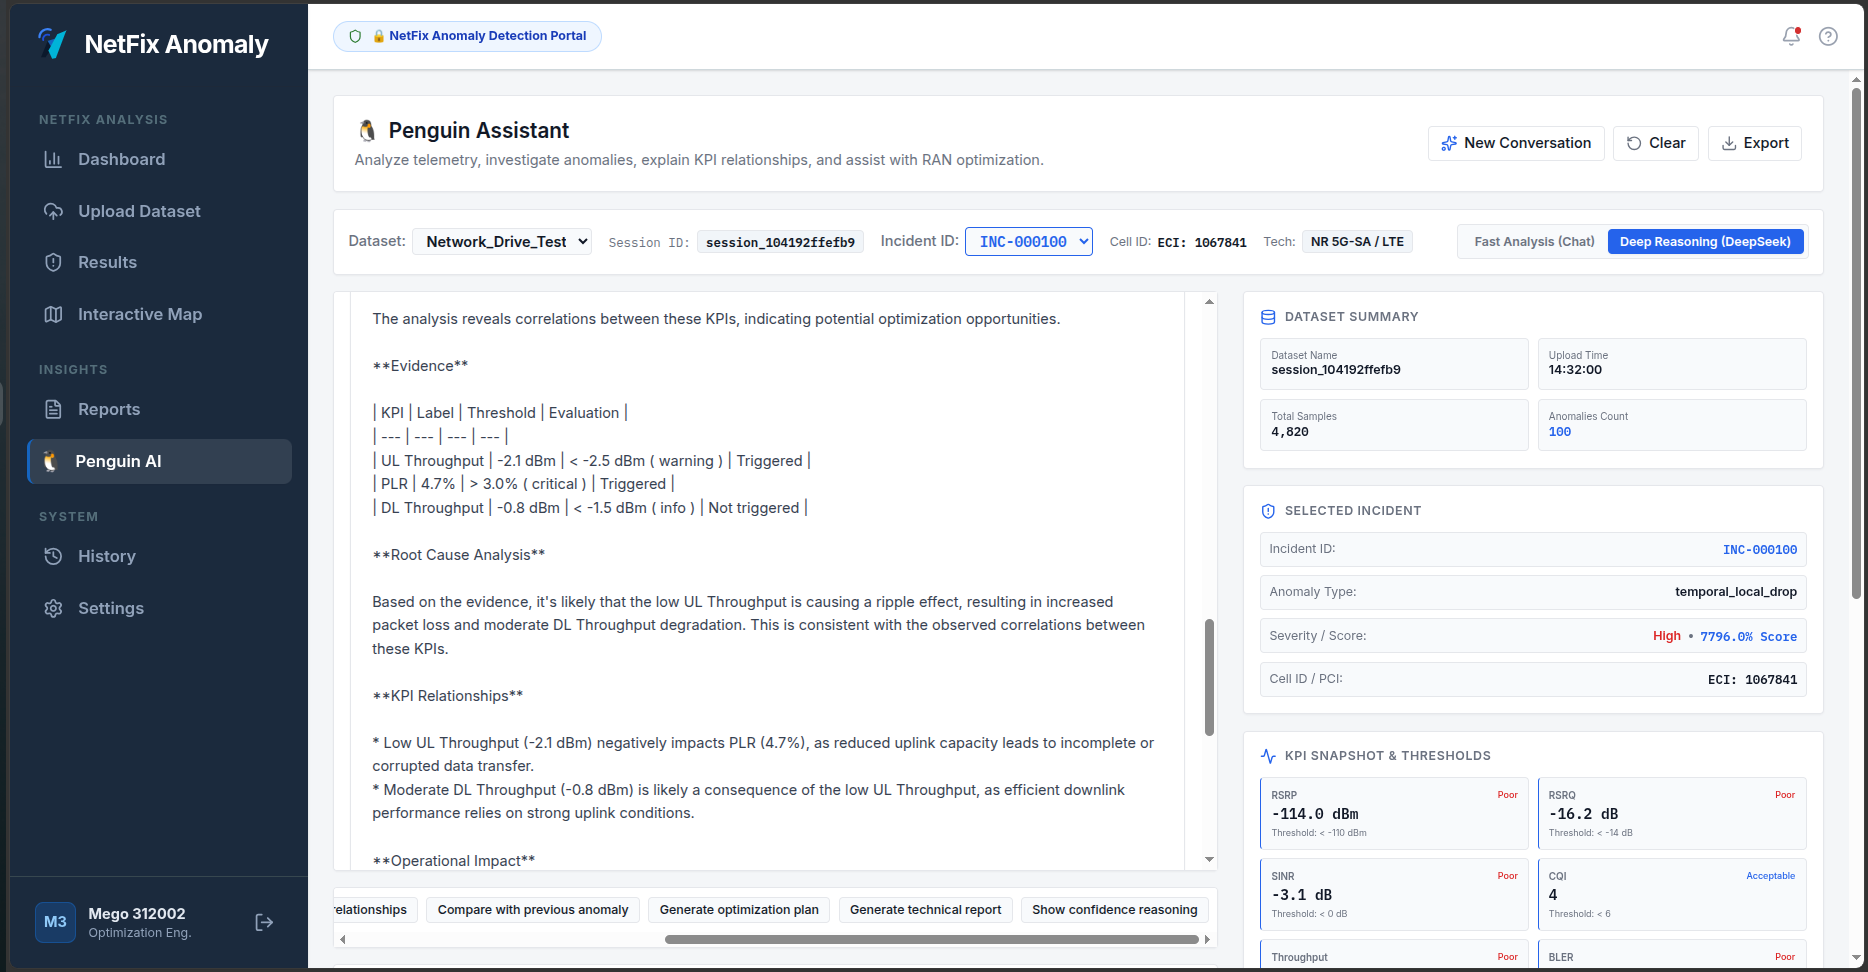
\includegraphics[width=\linewidth]{Screenshot from 2026-08-11 20-52-46.png}
  \caption{Evidence and diagnosis.}
\end{subfigure}\hfill
\begin{subfigure}[t]{0.32\textwidth}
  \centering
  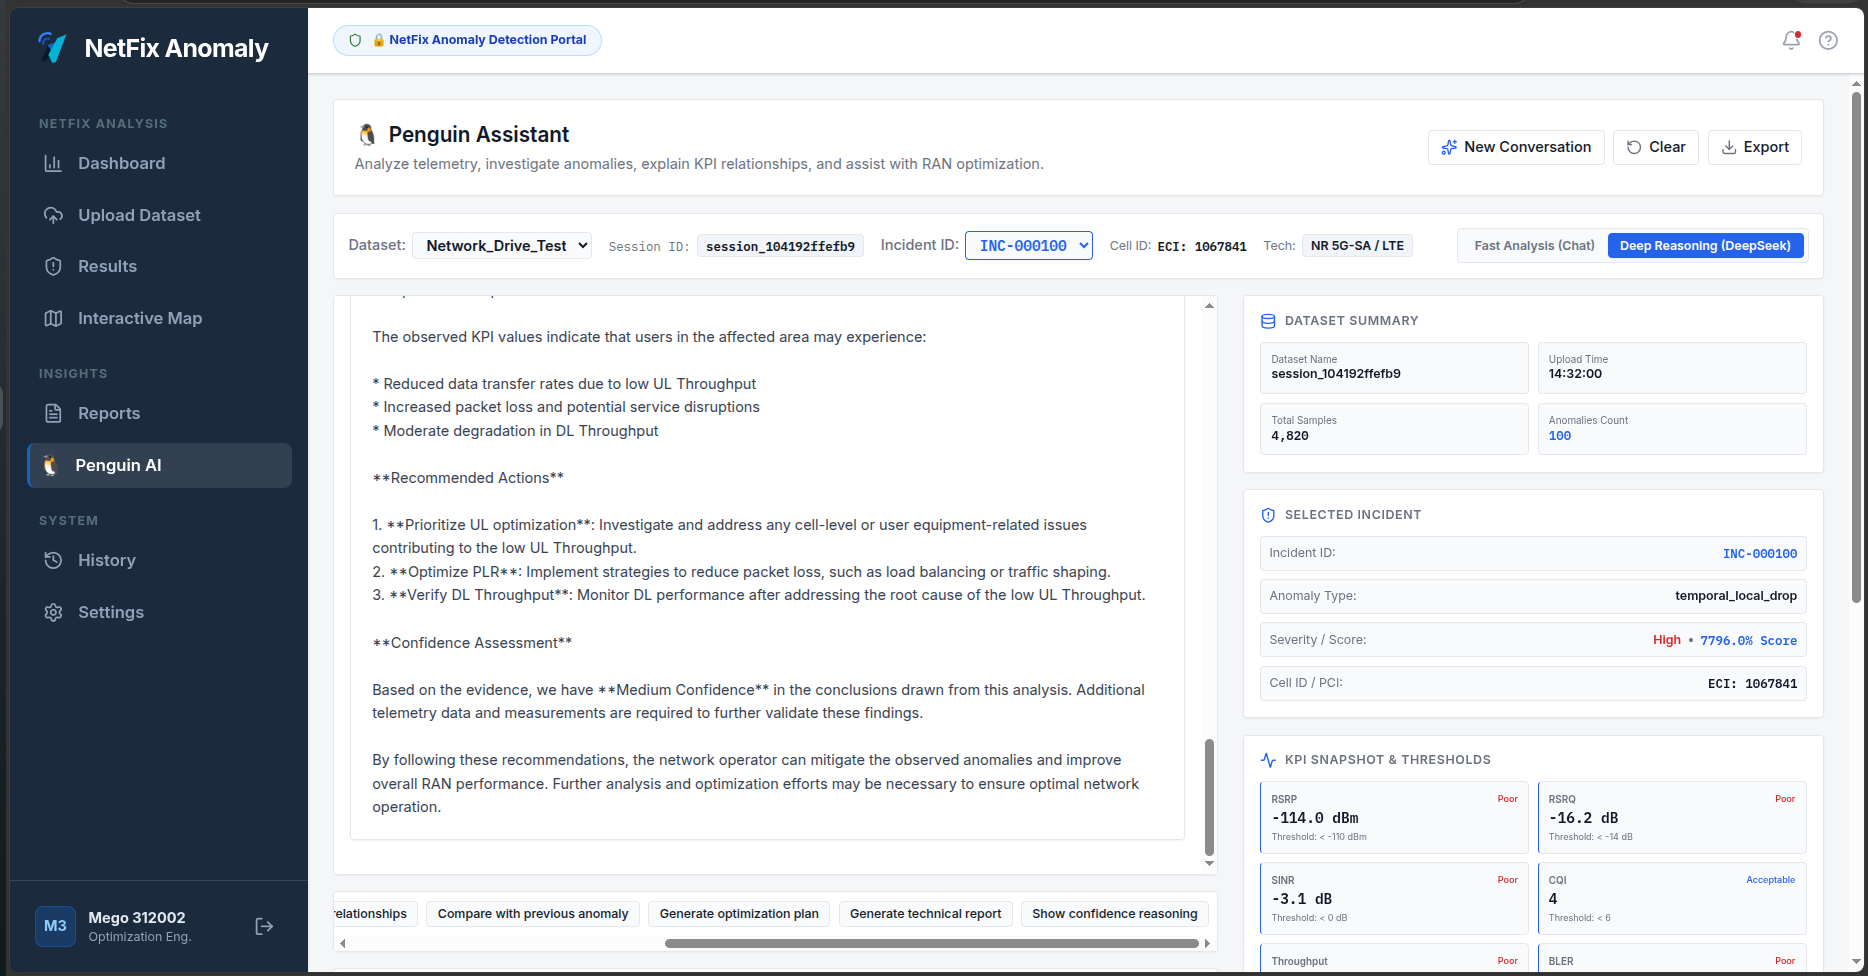
\includegraphics[width=\linewidth]{Screenshot from 2026-08-11 20-52-49.png}
  \caption{Actions and confidence.}
\end{subfigure}
\caption{Automated technical-report generation sequence.}
\label{fig:ug-penguin-report}
\end{figure}

\begin{figure}[H]
\centering
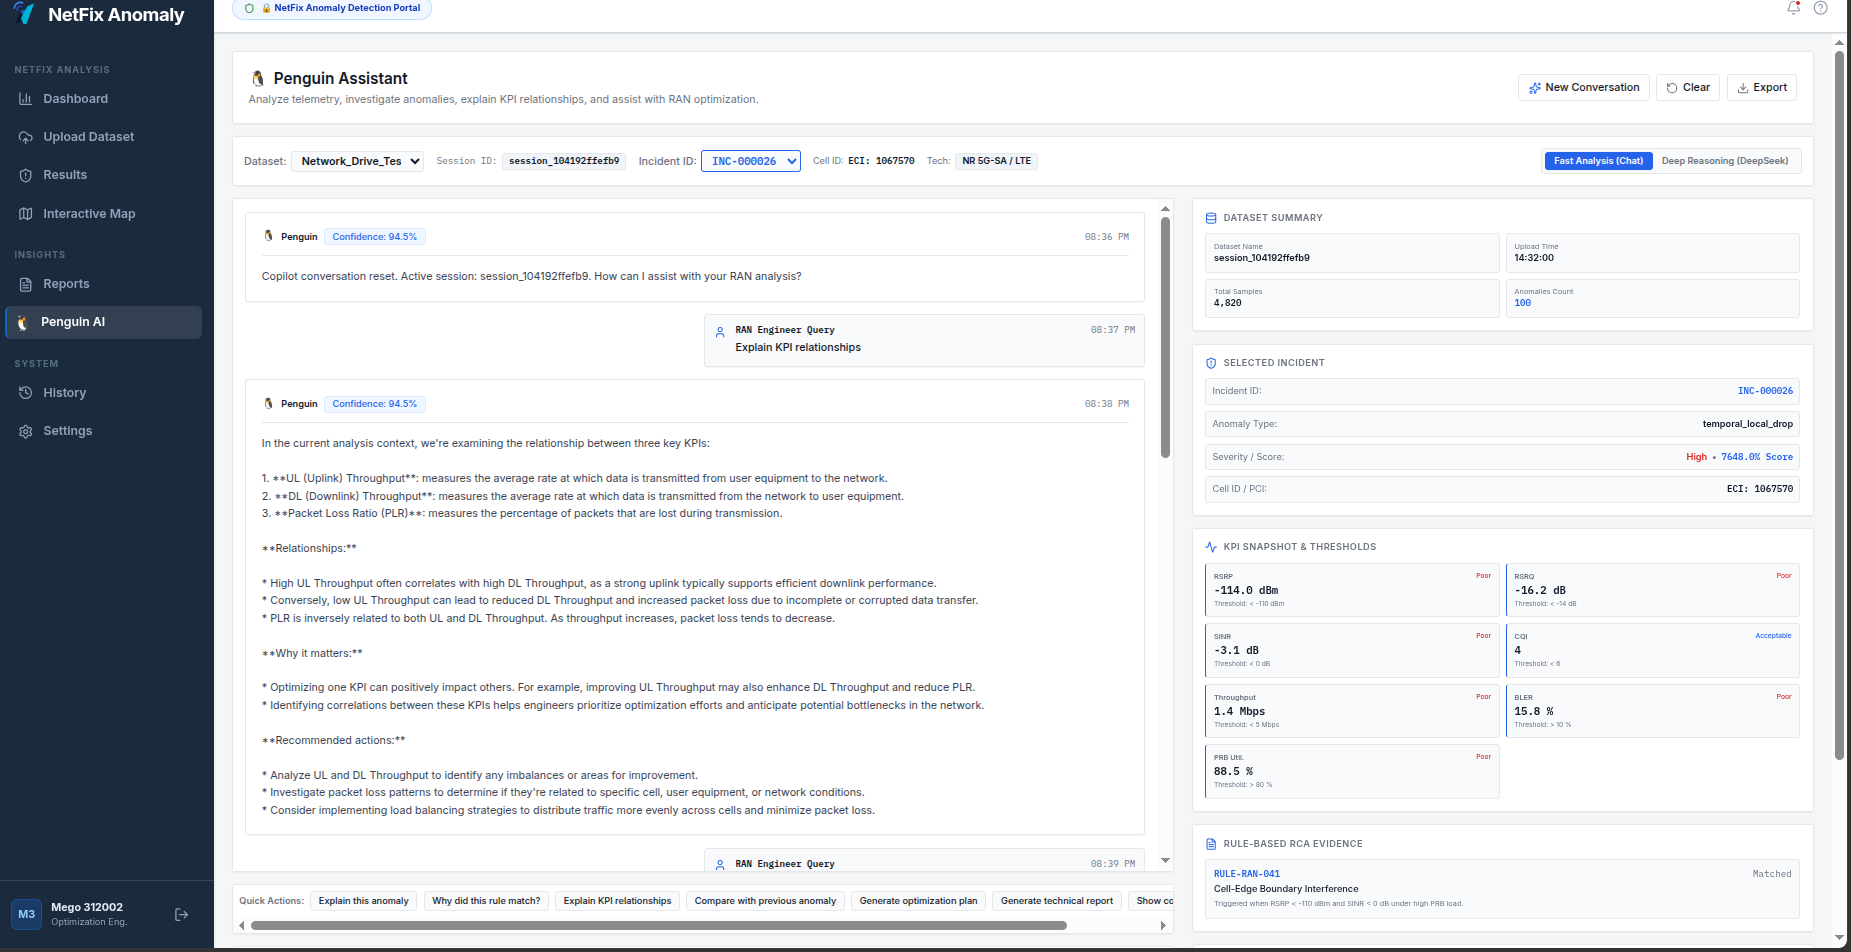
\includegraphics[width=0.90\textwidth]{Screenshot from 2026-08-12 14-39-31.png}
\caption{Penguin AI analyzing an incident matched to RULE-RAN-041 Cell-Edge Boundary Interference.}
\label{fig:ug-penguin-cell-edge}
\end{figure}
\FloatBarrier

\subsubsection{Assistant controls and execution modes}
\begin{itemize}
  \item \textbf{Conversation controls:} New Conversation, Clear, and Export.
  \item \textbf{Context bar:} active dataset, session, incident, cell, and radio technology. The illustrated context includes \texttt{Network\_Drive\_Test}, \texttt{session\_104192ffefb9}, \texttt{INC-000100} / \texttt{INC-00026}, \texttt{ECI: 1067841}, and \texttt{NR 5G-SA / LTE}.
  \item \textbf{Fast Analysis (Chat):} Llama 3.1 8B for direct engineering dialogue.
  \item \textbf{Deep Reasoning (DeepSeek):} DeepSeek R1 8B for extended reasoning workflows.
\end{itemize}

\subsubsection{Supported workflows}
\begin{itemize}
  \item \textbf{Explain KPI relationships} --- in the illustrated example, Penguin reports 94.5\% confidence and explains the interaction among UL throughput, DL throughput, and Packet Loss Ratio (PLR), including the effect of delayed TCP ACKs and TCP-window reduction on DL performance.
  \item \textbf{Generate technical report} --- creates session metadata, executive summary, evidence table, RCA, recommended actions, and confidence assessment. The sample report identifies \texttt{session\_104192ffefb9}, date \texttt{2023-02-20}, and author \texttt{Penguin, AI Engineering Copilot}; it highlights Low UL Throughput (-2.1 dBm), High PLR (4.7\%), and Moderate DL Throughput (-0.8 dBm), then recommends UL optimization, PLR/load-balancing actions, and post-remediation DL verification.
  \item \textbf{Explain this anomaly / Why did this rule match?} --- grounds the answer in the active incident and deterministic RCA evidence.
  \item \textbf{Compare with previous anomaly / Generate optimization plan / Show confidence reasoning} --- provides one-click investigation prompts.
\end{itemize}

\subsubsection{Context and telemetry sidebar}
The right-side context panel keeps the active data and engineering thresholds visible while the assistant responds. The illustrated dataset summary shows \textbf{4,820 samples} and \textbf{100 anomalies}; the selected-incident card displays \texttt{temporal\_local\_drop}, Cell \texttt{ECI: 1067841}, and the UI severity / score string \texttt{High • 7796.0\% Score}.

\begin{table}[H]
\centering
\small
\begin{tabularx}{0.88\textwidth}{L{2.7cm} L{2.5cm} Y}
\toprule
\textbf{KPI} & \textbf{Displayed value} & \textbf{Displayed threshold / state} \\
\midrule
RSRP & -114.0 dBm & Poor; threshold $< -110$ dBm \\
RSRQ & -16.2 dB & Poor; threshold $< -14$ dB \\
SINR & -3.1 dB & Poor; threshold $< 0$ dB \\
CQI & 4 & Acceptable; threshold $< 6$ \\
Throughput & 1.4 Mbps & Poor; threshold $< 5$ Mbps \\
BLER & 15.8\% & Poor; threshold $> 10\%$ \\
PRB utilization & 88.5\% & Poor; threshold $> 80\%$ \\
\bottomrule
\end{tabularx}
\caption{Example KPI snapshot and thresholds displayed beside Penguin AI.}
\label{tab:penguin-kpi-context}
\end{table}

The same sidebar displays the matched deterministic RCA evidence, for example \texttt{RULE-RAN-041 Cell-Edge Boundary Interference}, so the LLM response remains connected to visible engineering evidence.

% ---------------------------------------------------------
\subsection{Module 6: Session History and Audit Trail}
% ---------------------------------------------------------
The History page maintains an audit trail of platform analysis sessions (Figure~\ref{fig:ug-history}).

\begin{figure}[H]
\centering
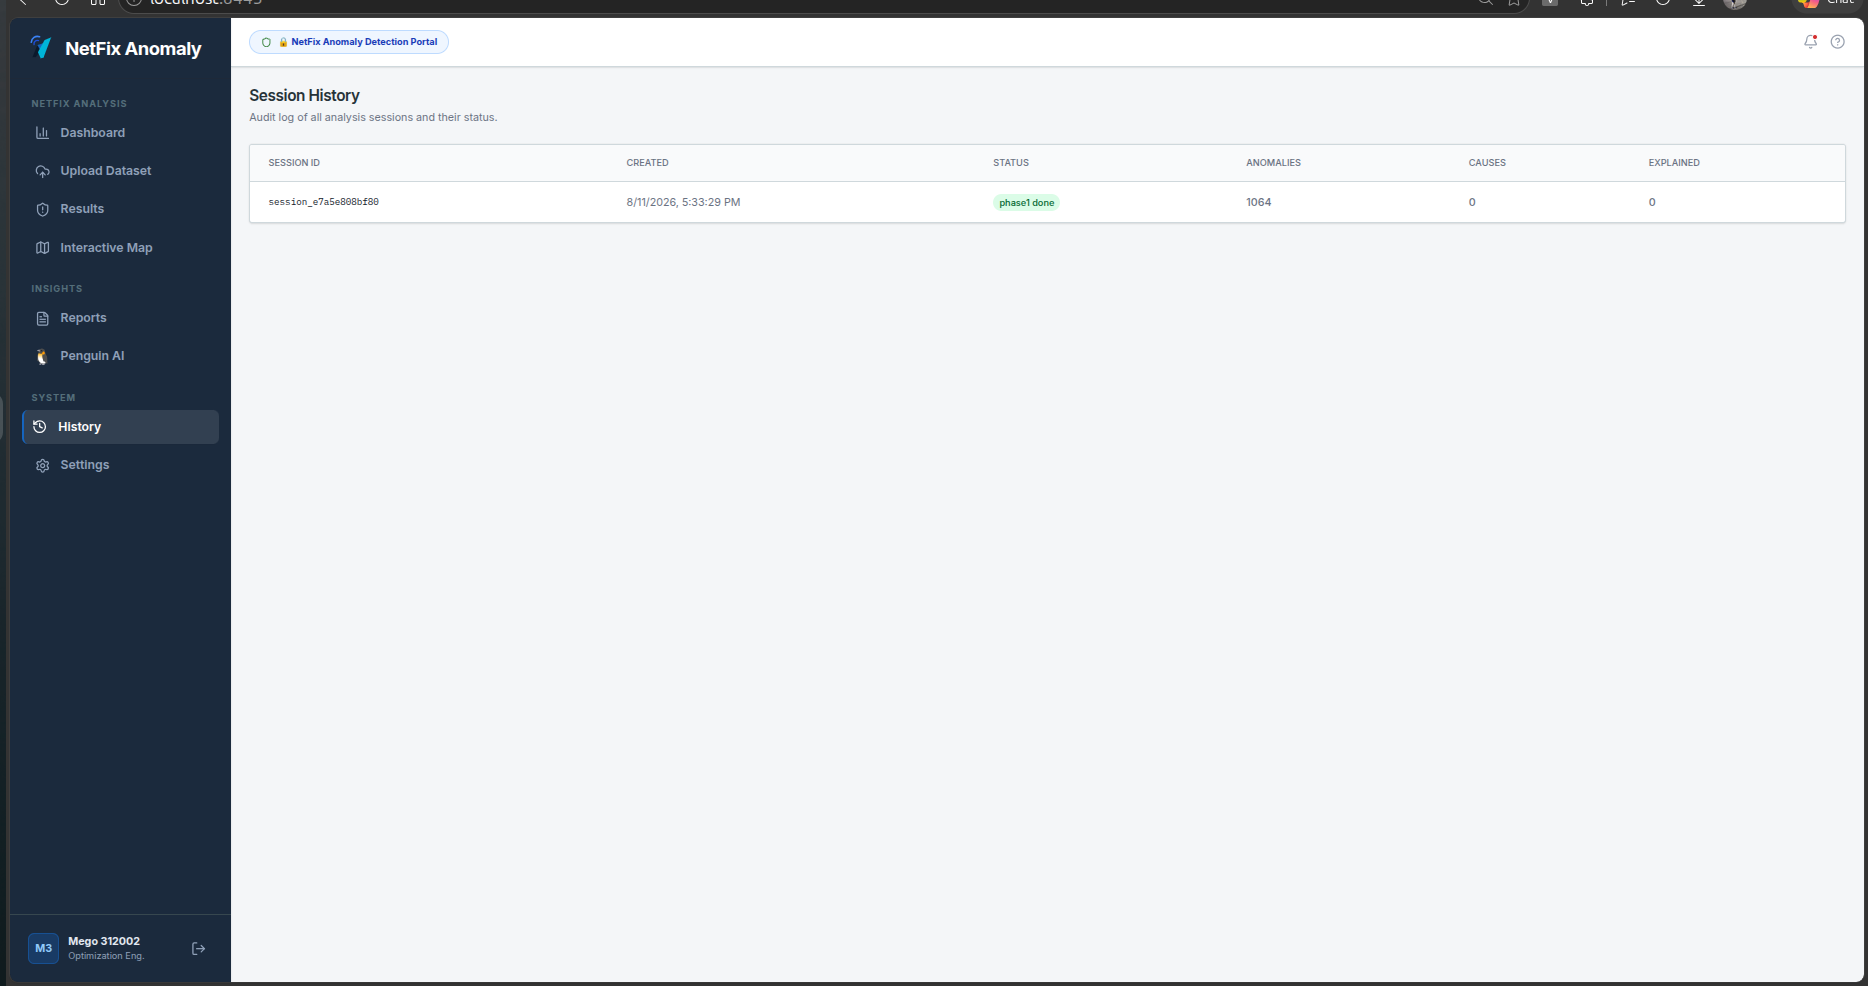
\includegraphics[width=0.96\textwidth]{Screenshot from 2026-08-12 14-39-40.png}
\caption{Session History showing timestamps, processing status, anomaly totals, and RCA progress.}
\label{fig:ug-history}
\end{figure}
\FloatBarrier

The table records \texttt{SESSION ID}, \texttt{CREATED}, \texttt{STATUS}, \texttt{ANOMALIES}, \texttt{CAUSES}, and \texttt{EXPLAINED}. For example, a completed Phase-1 session may show 1,064 anomalies before subsequent cause-matching and explanation fields are populated.

\newpage

% =========================================================
\section{5G Parameter Planning Portal (NetPulse)}
% =========================================================
\begin{guidebox}{Target user: 5G RF Planning Engineer / Network Deployment Specialist}
NetPulse supports workbook ingestion, clash auditing, automated bulk replanning, interactive site addition, assignment review, and export of deployment-ready planning parameters.
\end{guidebox}

\subsection{Step 1: Sign in and open the Planning workspace}
\begin{enumerate}
  \item Open \texttt{http://localhost:5173}.
  \item Select \textbf{Planning Engineer} on the sign-in screen.
  \item Click \textbf{Launch Portal}. The application routes to \textbf{Upload \& Plan} at \texttt{/np-upload}.
\end{enumerate}

\subsection{Step 2: Load a network-planning workbook}
\begin{enumerate}
  \item In \textbf{Upload \& Plan}, click \textbf{Upload Excel Workbook}.
  \item Load the raw or partially planned \texttt{.xlsx} file, for example \texttt{NR5G\_PCI\_RSI\_Planning\_raw.xlsx}.
  \item Alternatively, select one of the built-in system workbooks (\texttt{raw} or \texttt{final}).
  \item The backend parses sector geometry, azimuth, and the existing parameter assignments.
\end{enumerate}

\subsection{Step 3: Audit modulo conflicts and inspect the map}
\begin{enumerate}
  \item Open \textbf{Planning} to render the interactive site map and sector wedges.
  \item Open \textbf{Clashes} to inspect active conflicts:
  \begin{itemize}
    \item \textbf{PCI collision (hard):} same PCI assigned to adjacent sectors within the configured reuse distance.
    \item \textbf{Mod4 clash (hard):} same Modulo-4 index causing DMRS sequence overlap.
    \item \textbf{Mod3 / Mod30 warnings (soft):} PSS / SSS symbol-shift conflicts.
    \item \textbf{RSI collision (hard):} PRACH root-sequence contention.
  \end{itemize}
\end{enumerate}

\subsection{Step 4: Run automated bulk replanning}
\begin{enumerate}
  \item Return to \textbf{Upload \& Plan} and select \textbf{Bulk Replan Network}.
  \item The backend constraint solver processes the sectors and reassigns non-conflicting PCI values in $[0,1007]$ and RSI values in $[0,837]$.
  \item Verify that hard-clash counts fall to \textbf{0} before accepting the plan.
\end{enumerate}

\subsection{Step 5: Add a new site interactively}
\begin{enumerate}
  \item Open \textbf{Add Site}.
  \item Select the gNodeB location on the map or enter the coordinates manually.
  \item Define sector azimuths, for example $0^{\circ}$, $120^{\circ}$, and $240^{\circ}$.
  \item Click \textbf{Calculate Candidate Assignments} to generate valid PCI and RSI options.
  \item Choose the preferred assignment and click \textbf{Commit New Site}.
\end{enumerate}

\subsection{Step 6: Review and export the engineering plan}
\begin{enumerate}
  \item Open \textbf{Assignments} to review the complete network configuration table.
  \item Click \textbf{Export Excel Workbook (\texttt{.xlsx})} to download the final parameters for deployment / commissioning.
\end{enumerate}

\begin{warningbox}{Before exporting}
Confirm that all hard validation rules pass, review any remaining soft warnings, and verify that the assignment table reflects the intended site / sector configuration.
\end{warningbox}

% =========================================================
\section{Operational Notes}
% =========================================================
\begin{itemize}
  \item Use the role assigned to the engineer; role routing determines the default workspace.
  \item Keep dataset / workbook names descriptive so sessions can be identified later in History.
  \item Treat AI-generated explanations as engineering assistance; deterministic evidence, KPI values, standards references, and final engineer review remain visible in the workflow.
  \item Use session history and exported reports to retain an auditable record of analysis and planning actions.
\end{itemize}

\end{document}
